\documentclass[twocolumn]{article}
\usepackage[utf8]{inputenc}
\usepackage[linesnumbered,ruled,vlined]{algorithm2e} 
\title{Lab 1 \\ \small Fundamentals of regression and classification.}
\author{David Padilla Orenga\\ Ignacio Pastore Benaim}
\date{\today}   % You can use \date{\today}
\usepackage{biblatex}
% \addbibresource{references.bib}
\usepackage{graphicx}
\usepackage{hyperref}
\usepackage{color}
\usepackage{booktabs}
\usepackage{amsmath}

% Hyphen penalty
\hyphenpenalty=10000
\exhyphenpenalty=10000
\sloppy

\begin{document}

\maketitle

\section{Introduction}

The goal of this practical session is to train and evaluate various machine learning models for both regression and classification tasks using two datasets:

\begin{itemize}
    \item \textbf{YearPredictionMSD dataset:} Used for the regression task.
     This dataset contains audio features extracted from the Million Song Dataset,
      with the aim of predicting the release year of a song.
    \item \textbf{CIFAR-10 dataset:} Used for the classification task. The CIFAR-10 dataset contains 60,000 32x32 color images across 10 different classes, such as airplanes, cars, birds, and ships.
    \end{itemize}

The objectives are:
\begin{itemize}
    \item Train and evaluate different models to predict the year of a song using audio features.
    \item Train models on the CIFAR-10 dataset to classify images, 
    with a focus on using both raw pixel data and GIST descriptors for feature extraction.
    \end{itemize}

All the experiments, including model training, hyperparameter tuning,
and evaluations, were run locally on a MacOS machine with an M1 processor. 
The reported fitting and prediction times correspond to 
this specific hardware configuration. The local notebook containing the code is attached to this report.


In this report, we will detail the preprocessing steps, model selection, 
hyperparameter tuning, and evaluation metrics. Results for both tasks are analyzed, 
and conclusions are drawn based on model performance.
 
\section{Methodology}

\subsection{Regression Task: Year Prediction (Million Song Dataset)}
The YearPredictionMSD dataset consists of over 500,000 songs 
represented by 90 audio features extracted from each song. The target 
variable is the release year of each song.

\subsubsection{Data Splitting}
The dataset was split into training, validation, and test sets:
\begin{itemize}
    \item 81\% for training.
    \item 9\% for validation.
    \item 10\% for the final test.
\end{itemize}
Cross-validation was performed on the training set to select the best model.

\subsubsection{Exploratory Data Analysis}
We first explored the distribution of the target variable (year), 
noting the imbalance with more songs in recent years, as shown in Figure \ref{fig:year_distribution}.

\begin{figure}[h]
    \centering
    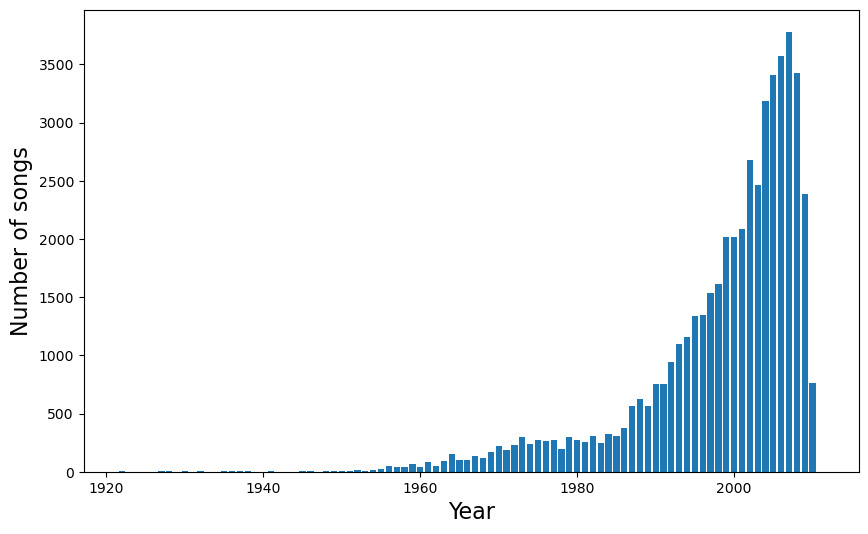
\includegraphics[width=0.8\linewidth]{images/songs/year_songs.png}
    \caption{Distribution of songs by year in the Million Song Dataset.}
    \label{fig:year_distribution}
\end{figure}


Additionally, we analyzed the correlations between features and the target variable 
to select promising features for modeling but we realized that it was better to apply PCA. 
Figure \ref{fig:correlation_features} shows correlations between the top features and the year of the song.

\begin{figure}[h]
    \centering
    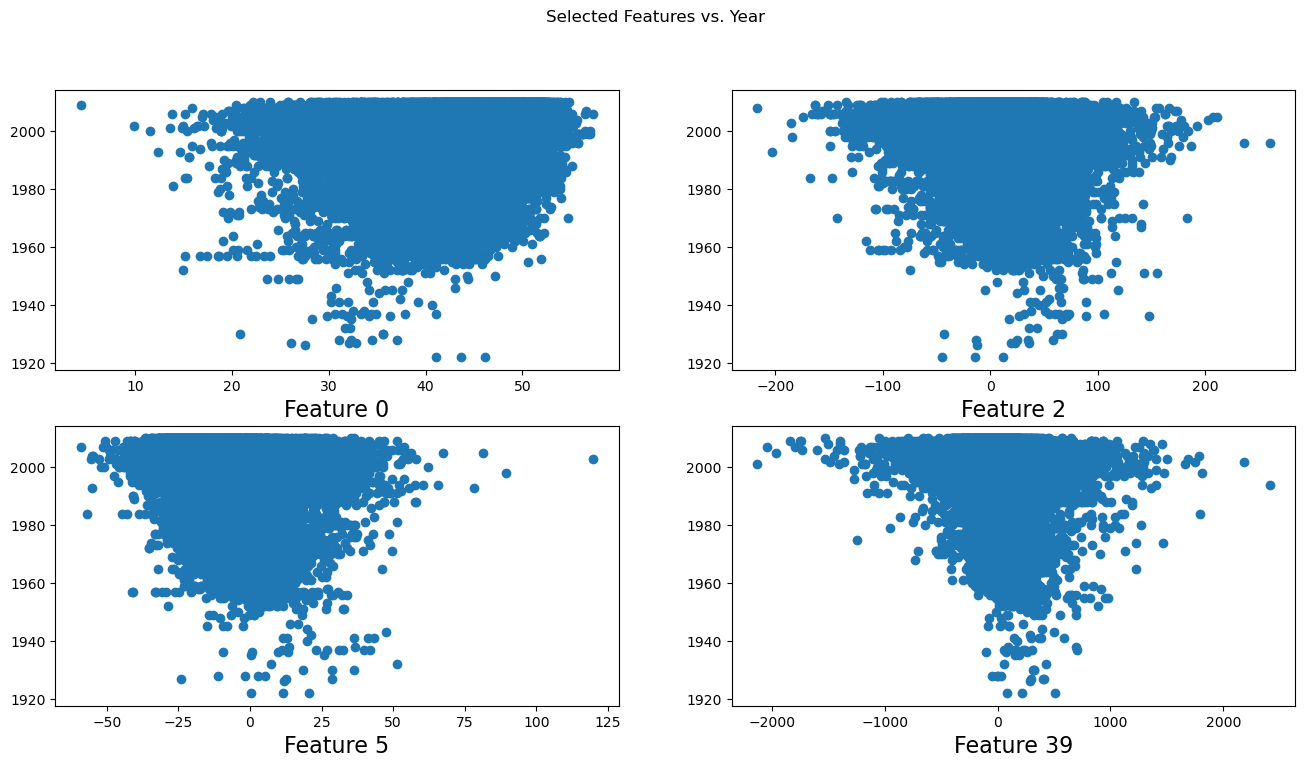
\includegraphics[width=0.95\linewidth]{images/songs/correlation_best_features.png}
    \caption{Selected features vs. year in the Million Song Dataset. Features where selected having 
    correlation with output $> 0.12$.}
    \label{fig:correlation_features}
\end{figure}

\subsubsection{Model Training and Hyperparameter Tuning}
We trained several regression models including:
\begin{itemize}
    \item Linear Regression
    \item Ridge Regression
    \item Lasso Regression
    \item ElasticNet
    \item Support Vector Regressor (SVR)
    \item Random Forest Regressor (RF)
    \item Gradient Boosting Regressor (GB)
\end{itemize}

Hyperparameters were tuned using GridSearchCV on the training and validation set,
 and models were evaluated using Mean Absolute Error (MAE), and Median Absolute Error (MedAE). 
 The results are detailed in the following tables (Section \ref{sec:regression_results}).

\subsection{Classification Task: CIFAR-10}

The CIFAR-10 dataset contains 60,000 images, evenly split across 10 classes. 
We tested different models for image classification, using both the raw pixel data and GIST descriptors.

\subsubsection{Data Preprocessing}
The CIFAR-10 dataset contains 60,000 images, evenly split across 10 classes. 
However, due to computational constraints, we limited our experiments to the first batch 
of 10,000 images from the dataset.

The dataset was split into training, validation, and test sets as follows:
\begin{itemize}
    \item 8,100 images (81\%) for training.
    \item 900 images (9\%) for validation.
    \item 1,000 images (10\%) for the final test.
\end{itemize}


We applied feature scaling to the raw pixel data and reduced its 
dimensionality using Principal Component Analysis (PCA) with 95\% variance retained. 
Afterward, GIST descriptors were computed for the same subset of images, allowing us to 
compare the performance of models trained on raw pixel data versus GIST-based features.

Although we performed comparisons on both the training and validation 
sets in the notebook, the reported comparison between raw pixel data and GIST descriptors 
is focused on the test set. The models were trained and evaluated using these two distinct 
feature sets to assess the effectiveness of each representation.

\subsubsection{Model Training and Hyperparameter Tuning}
Several classifiers were trained, including:
\begin{itemize}
    \item Support Vector Machines (SVM)
    \item Random Forest (RF)
    \item Multi-Layer Perceptron (MLP)
    \item K-Nearest Neighbors (KNN)
\end{itemize}
The models were tuned using GridSearchCV to find the best combination of hyperparameters.

Figures \ref{fig:success_classification} and \ref{fig:miss_classification} show 
successful and misclassified examples from the CIFAR-10 dataset.

\begin{figure}[h]
    \centering
    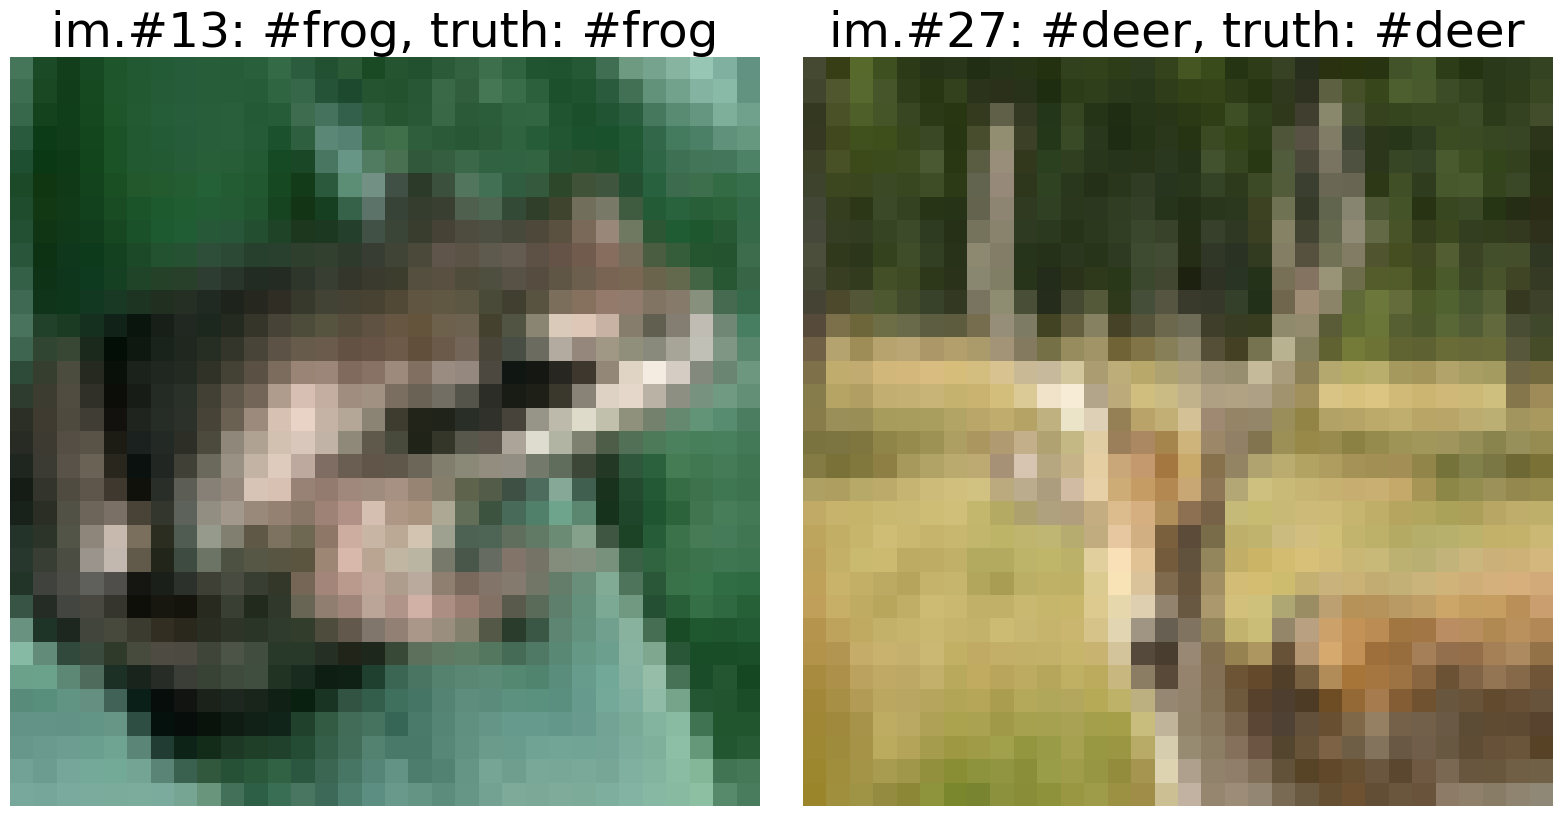
\includegraphics[width=0.95\linewidth]{images/CIFAR/scucess.png}
    \caption{Correctly classified images from CIFAR-10 dataset.}
    \label{fig:success_classification}
\end{figure}

\begin{figure}[h]
    \centering
    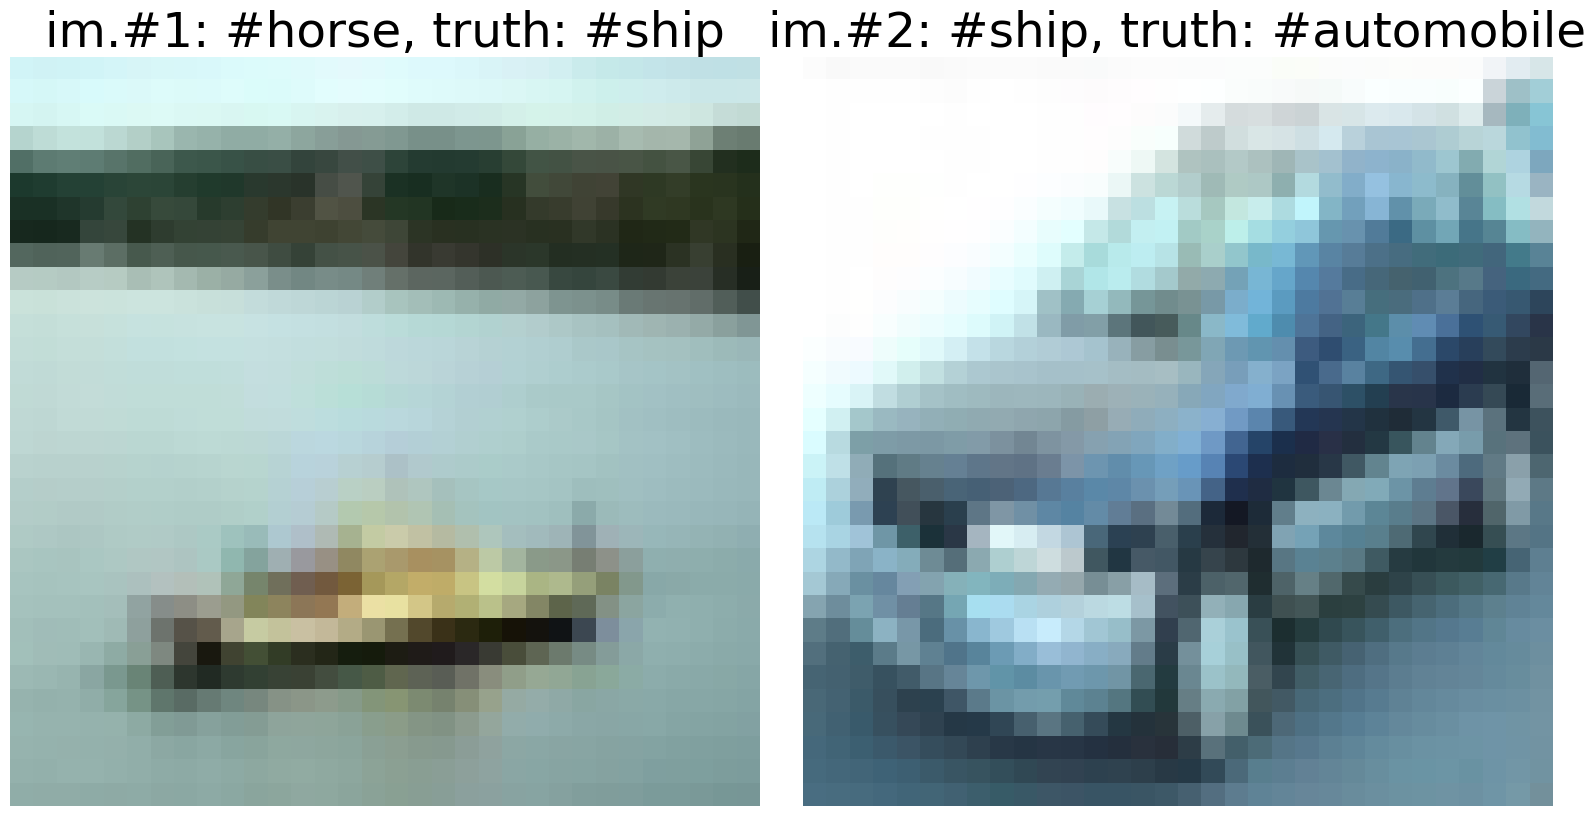
\includegraphics[width=0.95\linewidth]{images/CIFAR/missclasiffied.png}
    \caption{Misclassified images from CIFAR-10 dataset.}
    \label{fig:miss_classification}
\end{figure}

\section{Results}

\subsection{Regression Task: Year Prediction (Million Song Dataset)}
The table \ref{tab:year_song_screening} provides a screening of all the models.

\begin{table}
    \centering
    \caption{Screening of regression models with default parameters and PCA=0.95 for the year-song dataset.}
    \label{tab:year_song_screening}
    \begin{tabular}{|l|c|c|c|c|}
    \toprule
    Model & MAE & MedAE & Time (s) \\
    \midrule
    Linear  & 6.97 & 5.32 & 0.16 \\
    Ridge  & 6.97 & 5.32 & 0.08 \\
    Lasso  & 7.59 & 6.34 & 0.10 \\
    ElasticNet  & 7.43 & 6.11 & 0.09 \\
    Huber  & 6.73 & 4.68 & 0.60 \\
    RANSAC  & 25.34 & 18.20 & 0.43 \\
    SVR  & 6.15 & 3.97 & 125.17 \\
    RF  & 7.01 & 5.46 & 226.12 \\
    GB  & 6.77 & 5.09 & 84.34 \\
    KNN  & 6.68 & 4.80 & 0.07 \\
    \bottomrule
    \end{tabular}
\end{table}

The models were evaluated based on MAE (Mean Absolute Error) and MedAE (Median Absolute Error),
 as these metrics are more robust to outliers compared to RMSE. 
 The best-performing models were the Support Vector Regressor (SVR) 
 and Huber Regressor.

Due to time and computational constraints, we did not experiment with Huber Regressor using polynomial features, which might have further improved its performance. 
Additionally, K-Nearest Neighbors (KNN) was included in the comparison due to 
its simplicity and ease of implementation.

The following table summarizes the results of cross-validation for the trained models.

\begin{table}
    \centering
    \caption{Cross validation of best models. $ \text{Huber}(\alpha=0.001, \epsilon=1.35)$,
     $ \text{KNN}(n\_neighbors=7, p=2, \text{weights}=\text{'uniform'})$, 
     $ \text{SVR}(C=10.0, \gamma=\text{'scale'}, \text{kernel}=\text{'rbf'})$. 
    Time = time elapsed for all folds. Metrics are the mean over the 5 folds.}
    \label{tab:year_song_cross_validation}
    \begin{tabular}{|l|c|c|c|}
    \toprule
    Model & MAE & MedAE  & Time (s) \\
    \midrule
    Huber & 6.80 & 4.69  & 1.2 \\ 
    SVR & 6.01 & 3.89  & 960.0 \\
    KNN & 6.79 & 4.91  & 10.9 \\
    \bottomrule
    \end{tabular}
\end{table}

All the models in the cross validation step were selected for the final test, shown in Table \ref{tab:year_song_test}.

\begin{table}
    \centering
    \caption{Test performance of best models. $ \text{Huber}(\alpha=0.001, \epsilon=1.35)$, $ \text{KNN}(n\_neighbors=7, p=2, \text{weights}=\text{'uniform'})$, $ \text{SVR}(C=10.0, \gamma=\text{'scale'}, \text{kernel}=\text{'rbf'})$.}
    \label{tab:test_performance}
    \begin{tabular}{|l|c|c|c|c|c|}
    \toprule
    Model & MAE & MedAE & Fitting T(s) & Predicting T (s) \\
    \midrule
    SVR & 5.91 & 3.89 & 638.19 & 26.90 \\
    Huber & 6.76 & 4.67 & 0.91 & 0.00 \\
    KNN & 6.70 & 5.00 & 0.08 & 0.44 \\
    \bottomrule
    \end{tabular}
\end{table}


In summary, SVR and Huber stood out as the top performers, 
with KNN serving as reference.

\subsection{Classification Task: CIFAR-10}
For the classification task, the models were evaluated based on several metrics, 
including accuracy, precision, recall, and F1-score. The performance of the models was 
first assessed using a screening approach to identify potential candidates, followed by 
hyperparameter tuning through cross-validation. Finally, the best models were tested on 
the holdout test set to evaluate generalization.

\subsubsection{Model Screening}
The initial screening of models was performed using both raw pixel data and GIST
 descriptors to compare their effectiveness in representing image features for classification.
  The results from this screening process are summarized in Table \ref{tab:CIFAR_screening}, 
  where only the metrics for the raw pixel data are shown. 

\begin{table}
    \centering
    \caption{Screening of classification models with default parameters and PCA=0.95 for the CIFAR-10 dataset.}
    \label{tab:CIFAR_screening}
    \begin{tabular}{|l|c|c|c|c|c|}
    \toprule
    Model & Acc. & F1 & Prec. & Rec. & Fitting T. (s) \\
    \midrule
    LR & 0.37 & 0.37 & 0.37 & 0.37 & 21.98 \\
    SVM & 0.46 & 0.46 & 0.46 & 0.46 & 29.40 \\
    KNN & 0.31 & 0.30 & 0.39 & 0.31 & 28.11 \\
    RF & 0.35 & 0.34 & 0.35 & 0.34 & 40.01 \\
    MLP & 0.39 & 0.39 & 0.39 & 0.39 & 56.40 \\
    \bottomrule
    \end{tabular}
\end{table}

From the screening, we observed that models trained on raw pixel data showed significantly
 better performance, with the Support Vector Classifier (SVC) and MLP among the top-performing models. 
 Models trained on GIST descriptors struggled to achieve comparable accuracy due
  to the lower dimensionality and feature representation limitations of the descriptors.

\subsubsection{Cross-Validation Results}
After the screening, we performed hyperparameter tuning using GridSearchCV on the validation and training 
set to find the best hyperparameter combinations for the top-performing models.
 The results of this cross-validation process are shown in Table \ref{tab:CIFAR_cross_validation}, 
 where models were evaluated across 5 folds for stability and generalization.

\begin{table}
    \centering
    \caption{Cross-validation performance of classification models wit PCA=0.95.
     $ \text{SVC}(C=1$), $ \text{MLP}(hidden layers =(100,))$.  
     Time = cross-validation time over 5 folds.}
    \label{tab:CIFAR_cross_validation}
    \begin{tabular}{|l|c|c|c|c|c|}
    \toprule
    Model & Acc. & F1 & Prec. & Rec. & T.(s) \\
    \midrule
    SVC & 0.4581 & 0.4561 & 0.4587 & 0.4580 & 87.13 \\
    MLP & 0.3786 & 0.3784 & 0.3795 & 0.3782 & 82.19 \\
    \bottomrule
    \end{tabular}
\end{table}

The SVC with a radial basis function (RBF) kernel consistently performed the best across 
different folds, achieving the highest average accuracy. Also MLP performed similarly, 
but SVC was elected for testing due to computational and time constraints.
GIST-based models generally showed lower cross-validation scores.

\subsubsection{Test Set Results}
Finally, SVC was evaluated on the test set. Table \ref{tab:CIFAR_test_results} 
presents the final performance over raw pixel data and GIST descriptors. There is a clear 
improvement in performance when using raw pixel data. This could be due to the fact that
we are using a subset of the dataset, and the GIST descriptors may not be able to capture
the necessary information for classification.

\begin{table}
    \centering
    \caption{Test performance of SVC models over the CIFAR-10 dataset. $\text{SVC + G = SVC + GIST}$. Both $\text{SVC}(C=1)$. $SVC + G()$ without PCA.}
    \label{tab:test_svc_performance}
    \begin{tabular}{|l|c|c|c|c|c|}
    \toprule
    Model & Acc. & F1 & Prec. & Rec. & Fit. T.(s)\\
    \midrule
    SVC & 0.47 & 0.46 & 0.46 & 0.46 & 43.91\\
    $SVC + G$  & 0.25 & 0.24 & 0.24 & 0.25 & 7.63 \\
    \bottomrule
    \end{tabular}
\end{table}


\section{Conclusion and Discussion}
In this report, we evaluated several machine learning models for both regression and classification tasks.

\subsection{Regression: Year Prediction Task}
For the YearPredictionMSD dataset, we found that the Support Vector Regressor (SVR) 
performed the best, achieving a Mean Absolute Error (MAE) of 5.91 years. 
Despite the strong performance of SVR, it was computationally expensive, making it less practical for large-scale applications.

K-Nearest Neighbors (KNN) was also evaluated and selected 
for its simplicity and ease of implementation. While it did not outperform SVR, 
KNN provided a practical baseline with acceptable performance for comparison.

RANSAC, on the other hand, struggled significantly with the complexity and outliers in the dataset, 
resulting in poor overall performance.

  \subsection{Classification: CIFAR-10 Task}
  In the CIFAR-10 classification task, 
  models trained on raw pixel data consistently outperformed those trained on GIST descriptors. 
  The best-performing model, SVC with an RBF kernel, achieved an accuracy of 47\%.
   However, it was observed that GIST descriptors, while faster to train on, r
   esulted in a significant loss of classification accuracy.
  
  A possible explanation for this drop in performance 
  when using GIST descriptors is the smaller subset of images used in this experiment. 
  With only 10,000 images (instead of the full 60,000), the GIST descriptors may not 
  have captured enough variability in the dataset, limiting their effectiveness as feature representations.
  
  Future work could explore deep learning models such as 
  Convolutional Neural Networks (CNNs) for image classification, 
  as they are known to perform better on image datasets like CIFAR-10 by 
  automatically extracting more robust features. Additionally, training with 
  the full CIFAR-10 dataset may help improve the performance of models based on GIST 
  descriptors, as the larger sample size would allow for better feature extraction and learning.


\end{document}


